% ----------------------------------------------------------------------------------------
% CHAPTER TITLE
% ----------------------------------------------------------------------------------------
\chapter{Selected Recent Works}\label{selrecworks}
\lhead{\chaptertitlename\ \thechapter. \emph{Selected Recent Works}}
% ----------------------------------------------------------------------------------------

This chapter describes a selection of designs from the past few years by makers in electronic music. These designs relate in many ways to the concept of open source as it was discussed in the last chapter, that is, devices which in their creation process create some amount of freely available information that enables future developers.

They were selected because they serve as examples of progress in a modern vision of electronic music hardware and its related approach to composition. Either through ideas or implementations, they constitute a compelling progress in the field. Documentation (either public, academic, or reverse-engineered) for these devices was collected and analyzed, and this chapter is a series of case studies explaining how these works were developed and why they are important in our context of open design. 

As will be detailed, broad categories are identified and used to group some of the projects. 

\section{Devi Ever FX and Dwarfcraft Devices}

Devi Ever FX was initially ran by a Devi Ever, who designed a long list of different distortion pedals before leaving the business to Louise and Ben Hinz. Devi was particularly appreciated in the online pedal DIY scene for her willingness to share and discuss audio circuit designs. 

One of these designs in particular appears as interesting: the \emph{improbability drive}. It was selected for the way this particular project is approached by community, and the ubiquitous role of fuzz pedals in the development of a diy practice. Paraphrasing an earlier citation from Collins, the internet did explode, and with it, a thousand fuzz designs did become available. For some, they were a way to waste time and money, for others, these became the foundation for multiple businesses. 

\subsection{the improbability drive}

Devi Ever (under the new Hinz ownership) currently sells 23 different designs of guitar effect pedals (mainly focused around distortions, overdrives or fuzzes), while its ``outdated'' page names 30 additional discontinued models. 

The Improbability Drive's circuit was first posted by Devi Ever herself on the freestompboxes.org forum, notorious for its avid reverse engineering community of musicians and diy experimenters. Although the original schematic is no longer

``http://freestompboxes.org/viewtopic.php?f=7&t=18157&hilit=devi+ever+fx''

\section{CMOS synthesis: modern incarnations}

\begin{quote}
	
	We can make our ``1"-``0" decisions into just about anything- a musical note, a test waveform, a measured and displayed value, a video presentation, a clock, a game, an industrial control, a toy, a microcomputer, an art form, a community information access service, or just about anything else you can dream up. All it takes is the right number of logic blocks properly connected to do the job.
	\citep[pp-7-8]{lancaster1988}
	
\end{quote}

\emph{Handmade Electronic Music} focuses much of its circuits around the Complementary-Silicon-Metal-Oxide (CMOS) family of integrated circuits. He acknowledges inspiration from Lancaster's CMOS cookbook, quoted above (personal conversation, 2015). In doing so, Collins acknowledges how powerful binary signals - an its continuous counterpart, the square wave - can be in relatively simple synthesis environments. Older examples abound: the Weird Sound Generator, a typical first synthesis project sold as a kit by Ray Wilson from the \emph{Music From Outer Space} website, relies on interconnected CMOS chips for its synthesis \citep{wilson2015}. Beavis Audio, an important diy music website, focuses one of its most interesting blog posts on this family of circuits, naming Collins as an influence \citep{beavis2015}. 

Although Collins is not the only source of these digital logic sound generators, the publication of his book has had a visible impact on many of the low-part-count synthesis circuits seen today. The two following examples exhibit particularly interesting and relevant semi-open projects. 

\subsection{Taylan Cihan: Porcupine (2013)}

Taylan Cihan's porcupine device is important because it is typical of experimenters who've grown comfortable with the various components of standard circuits (as exhibited in the improbability drive and \emph{Handmade Electronic Music}. After building things as the schematic tells you to, one can experiment with higher-level design and adapting the interface to make the experience of using the product more compelling. In this case, these are achieved by combining semi-standard circuits which illustrate introductory concepts of musical electronics, and by turning the design of an interface inside out to embrace the chaotic process from which it comes. 

Specifically, Cihan's circuit 

http://taylancihan.com/porcupine.html

\subsection{Dwarfcraft: the Robot Devil (2012)}

The relative simplicity of the device is here extremely relevant, as it has lead online community members to relate it to some circuits described in Nic Collins' \emph{Handmade Electronic Music}. 

``http://freestompboxes.org/viewtopic.php?f=7&t=18344&hilit=robot+devil''

The power of CMOS logic chips also serves as a segway into the wider topic of microcontroller synthesis. If Tristan Shone's system exhibited the power of arduinos in the context of controllers, numerous practitioners have also been developing instruments  In this case, embedded systems of various complexity have been used in innumerable synthesis projects, providing low fidelity audio outputs and high potential for customization. Sonically, these projects are very much indebted to the auditory product of CMOS chips combined with basic filtering and effects. 

\section{microcomputer systems}

\subsection{Tristan Shone: Author and Punisher}

A mechanical engineer and sculptor, Tristan Shone is the musician responsible for the one-man band \emph{Author and Punisher}. He released a first album in 2005, \emph{The Painted Army} \citep{shone,2005}, as he was developing his first set of instruments, the Drone machines. His website's subtitle is ``electromechanical destruction since 2004'' \citep{shone2004}.

	\begin{figure}[h!]
	  \caption{Shone's live setup around the release of the \emph{Drone Machines} album}
	  \centering
	    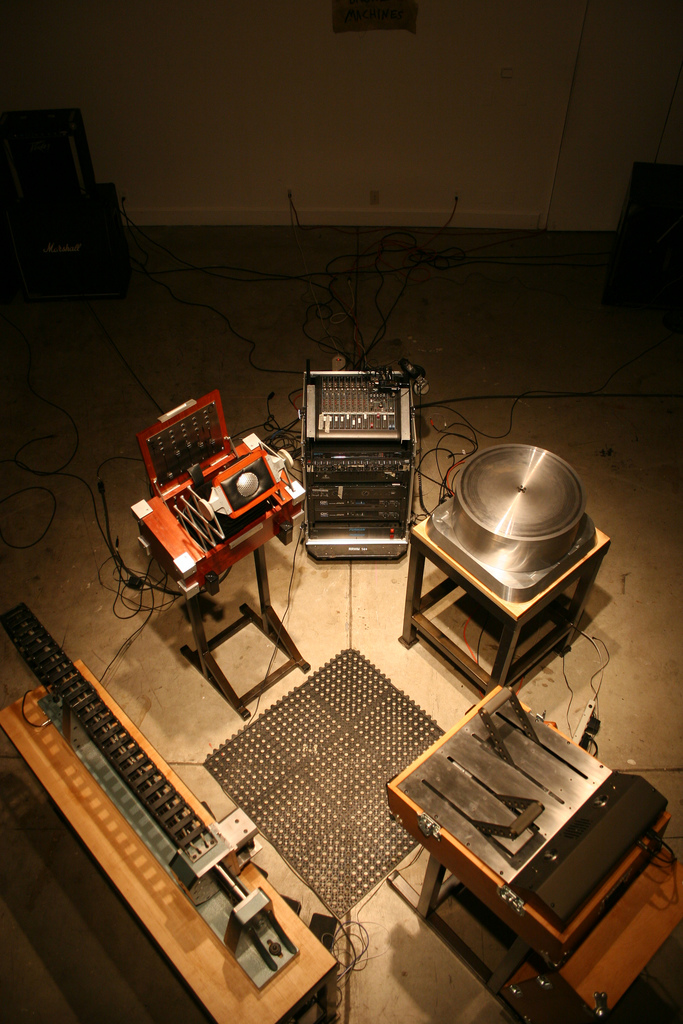
\includegraphics[width=.5\textwidth]{drone}
	\end{figure}
	
He has since released three more full-lengths relying increasingly on hardware he fabricated, in conjunction with a software sampling and synthesis system built around Ableton Live. Most of his devices have evocative names such as \emph{Linear Actuator}, \emph{Big Knobs} or \emph{Bellows}. 

	\begin{figure}[h!]
	  \caption{the \emph{Linear Actuator}}
	  \centering
	    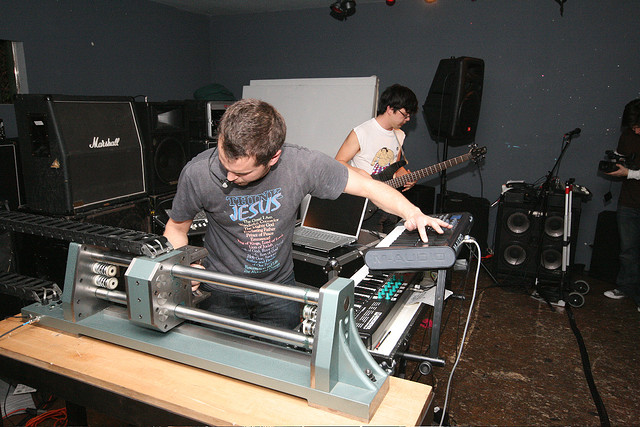
\includegraphics[width=1\textwidth]{linact}
	\end{figure}

	\begin{figure}[h!]
	  \caption{the \emph{Bellows}}
	  \centering
	    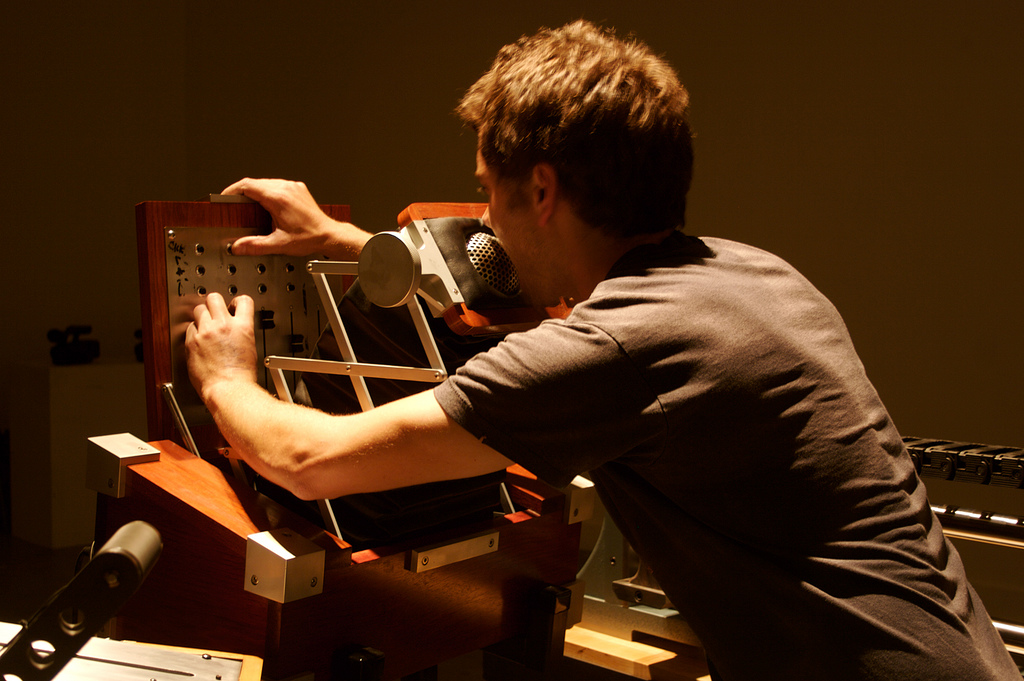
\includegraphics[width=1\textwidth]{bellows}
	\end{figure}

His experience with sculpture and mechanical engineering are clear, although discussing the matter with him makes it clear that he is ultimately making those because they seem like the best way to perform his music. Although he has grown to try and move away from the visual impact of his setup by collaborating with visual artists, his website still provides the curious with a combination of evocative live shots and technical diagrams. 

	\begin{figure}[h!]
	  \caption{a technical diagram for the \emph{Bellows} instrument}
	  \centering
	    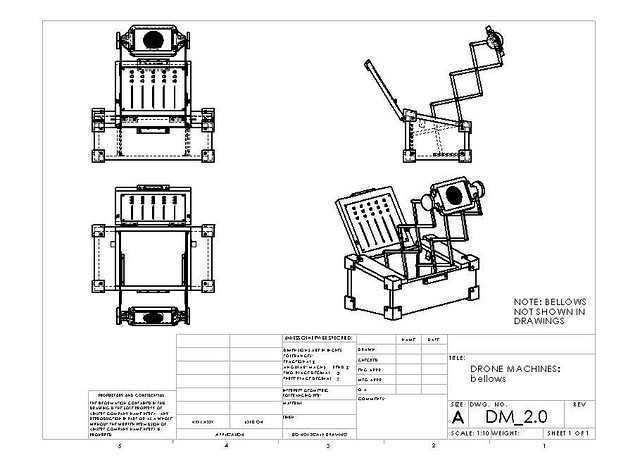
\includegraphics[width=1\textwidth]{bellowsdiag}
	\end{figure}
	
Most of these electromechanical devices act as controllers: they encode movement into a number using a microcontroller. This information is then fed into a computer, which triggers starts, changes and ends for specific sets of pre-composed sounds. 

Shone's microcontroller system is based on the arduino environment, which he uses with custom firmware developed by Dimitri Diakopoulos and featured at NIME in 2011 \citep{diakopoulos2011,diakopoulos2015} . This firmware modification turns a specific strands of the Arduino hardware (the Uno, Due and Mega 2560 boards) into a driverless device, enabling it to send MIDI data over USB without any more setup than a commercial USB-MIDI item. 

However, Shone's live setup is not just centered around controllerism. Shone describes himself as a ``lifelong beatboxer'' and in this context, he's devised a number of ways to detect, record and manipulate his voice \citep{shone2012}. He's currently developing a set of masks (documented on his website are the trachea quad mic, the dither mask, the drone mask and the mute mask), while his previous vocal interface is called the Headgear. That system was the topic of a tutorial written by Shone for the Make Magazine website \citep{shone2012}. 

http://makezine.com/magazine/make-22/seriously-heavy-metal/

\subsection{The Headgear system}

	\begin{figure}[h!]
	  \caption{the Headgear device, wired for operation}
	  \centering
	    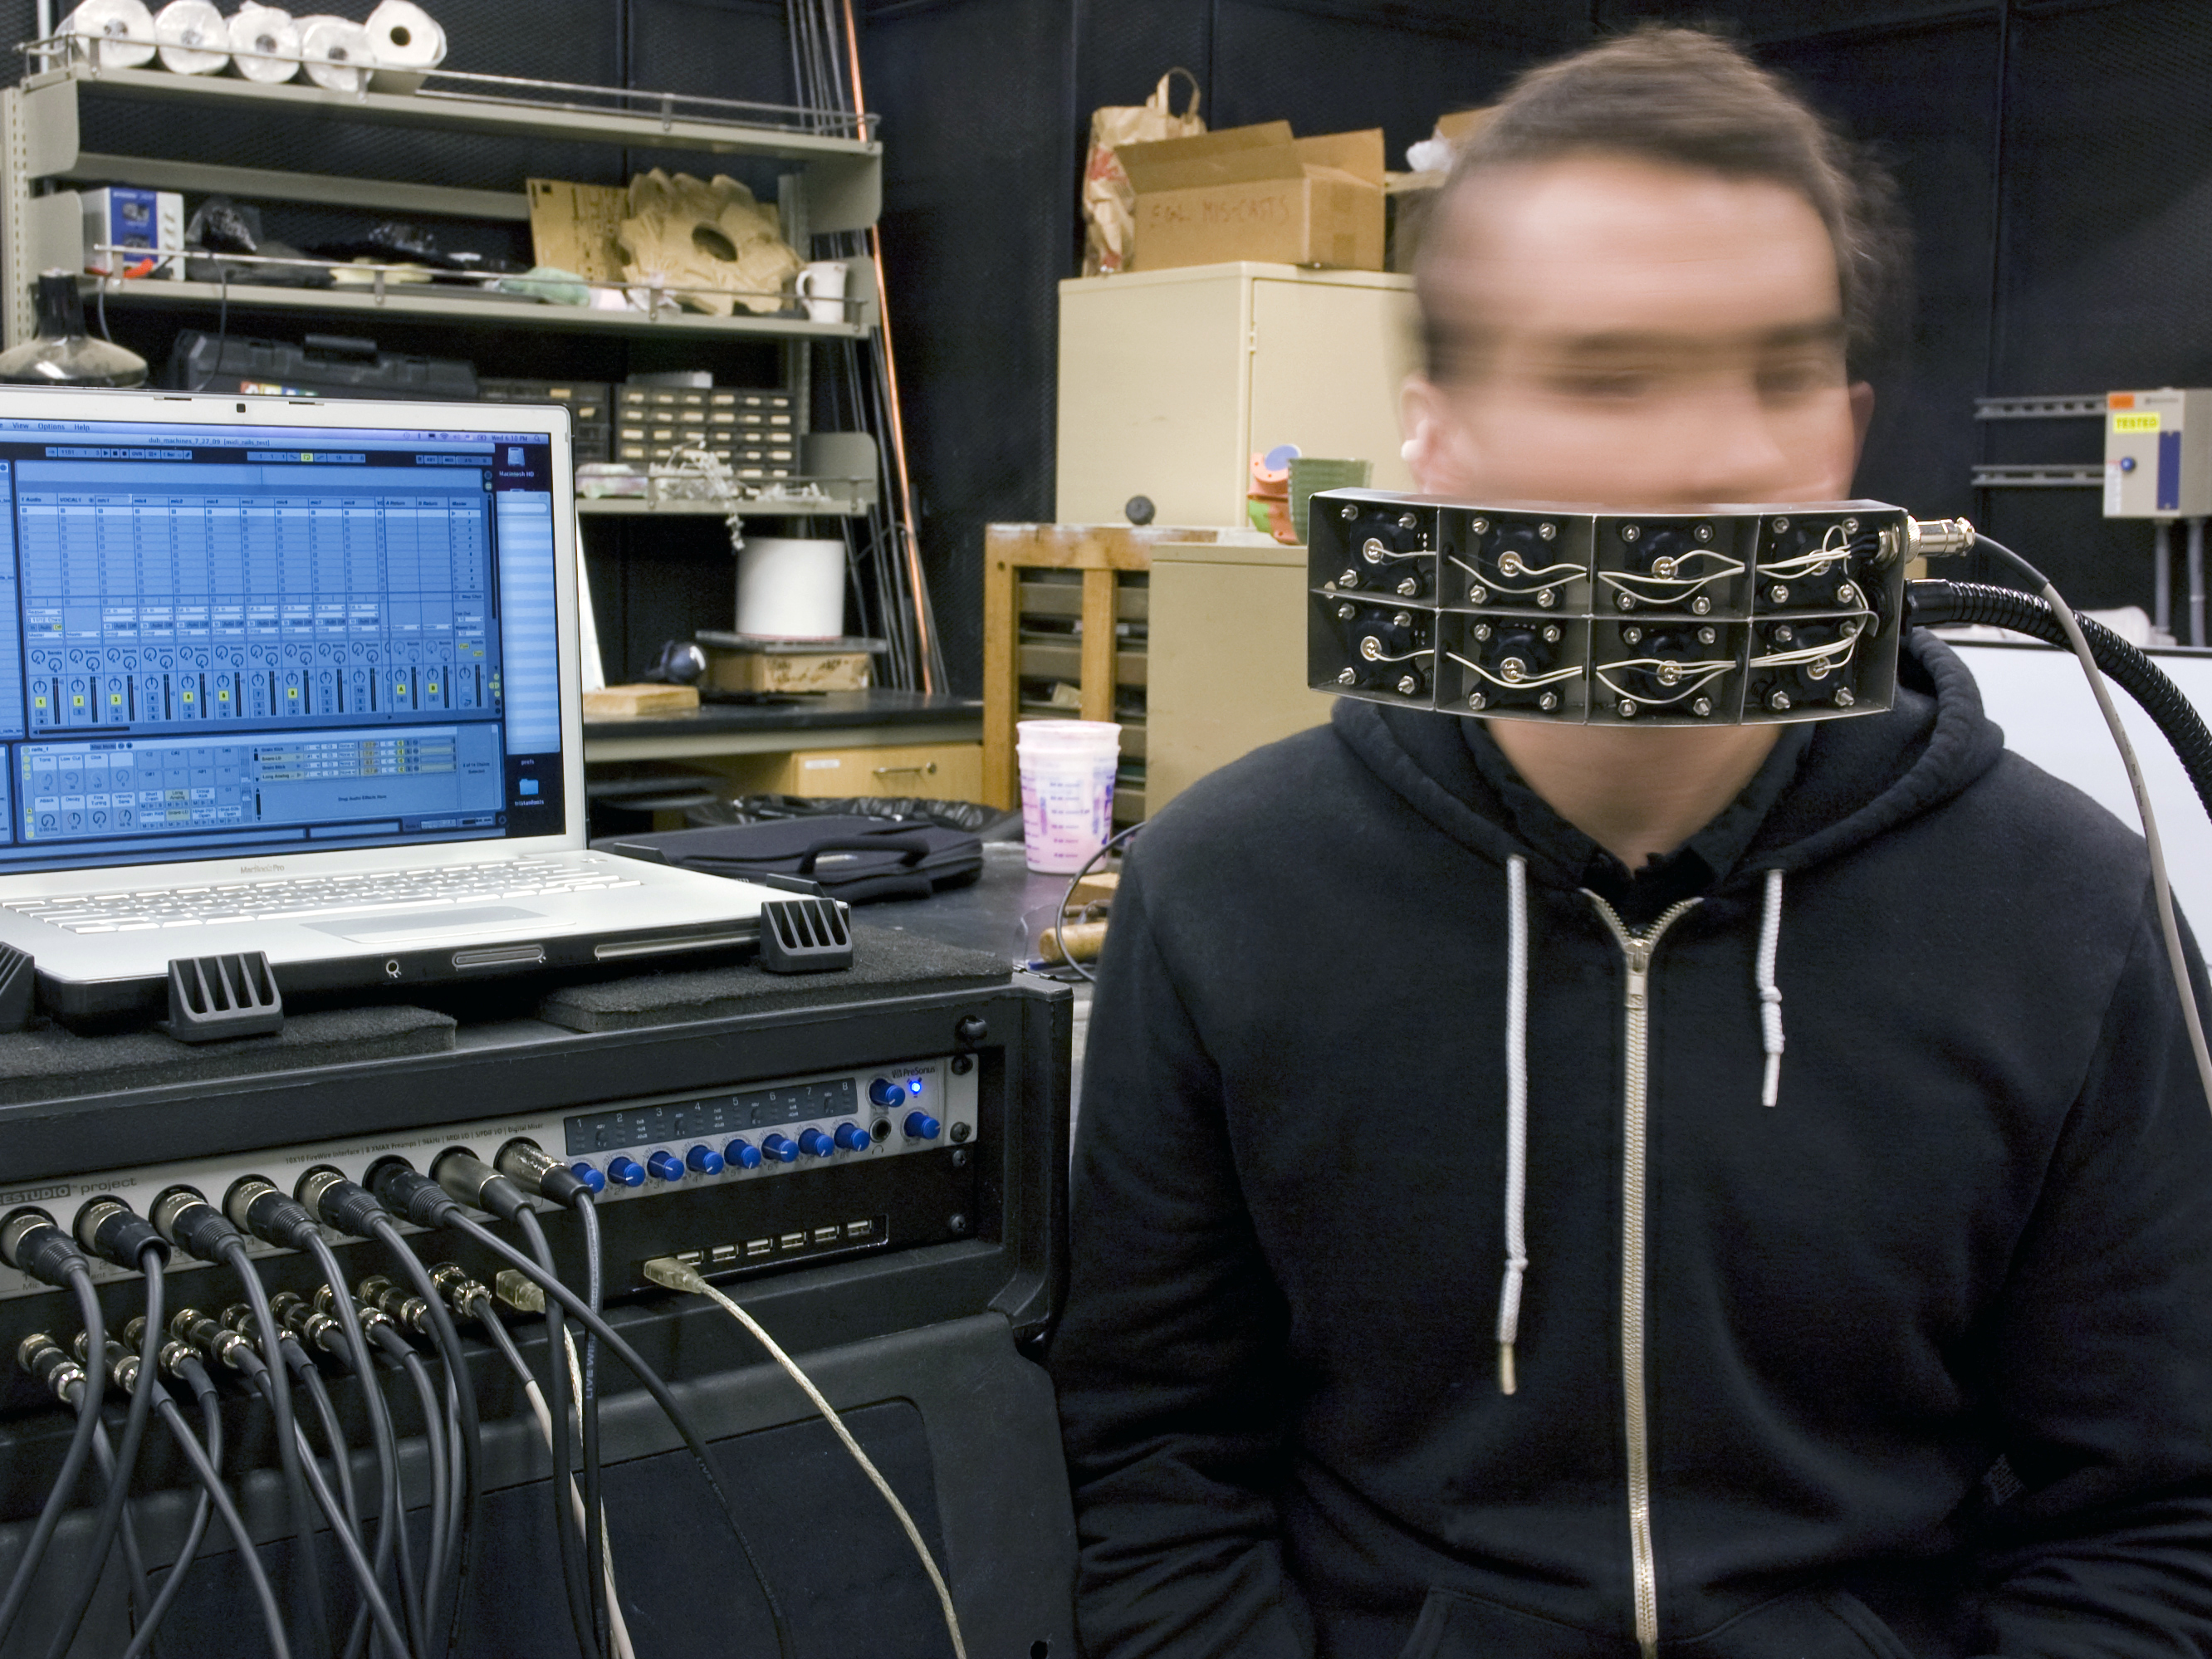
\includegraphics[width=1\textwidth]{headgear}
	\end{figure}

As can be expected in parallel with the rise of microcontrollers as interfaces for turning our environment into a source of control data, recent years have seen a number of initiatives turning accessible, general purpose computing devices into code-based synthesis engines. All these projects are the embodiment of their designer's curiosity, adapted to various degrees of interactivity for performance, composition or commercialisation. 

\subsection{Dan Snazelle, Snazzy FX: the ardcore}

The ardcore is in effect a reprogrammable lo-fidelity oscillator and control voltage generator packaged in a eurorack format and complemented by a set of freely available and editable programs. 

This project was developed by Darwin Grosse and Dan Snazelle. Darwin Grosse is a developper at Cycling `74, while Dan Snazelle is the owner and designer at Snazzy FX. Although the circuit itself isn't publicly available, all the arduino and avr code written by the developers and subsequent public is shared openly. 

https://github.com/eclectics/ardcore

https://github.com/darwingrosse/ArdCore-Code



\subsection{Tristan Perich and Loud Objects}

Tristan Perich's dual approach to music hardware is most clearly divided between his highly predetermined solo work, and the more chaotic performances he presents with Loud Objects. As part of the latter trio, he solders their instrument - a set of microcontrollers - as part of the performance, making the piece a circuit in the most Tudorian sense of the idea. 

As a composer, his work still relies on the binary output of microcontrollers, creating his ``one bit symphonies'' that have been presented as standalone pieces or along acoustic instruments in performances. 

http://vagueterrain.net/journal19/loud-objects/01

\subsection{Martin Howse: the dark interpreters}

Howse's esoteric psychogeophysics exploration is backed by a strong design and programming sense that's allowed him to turn some of his stranger ideas (booting a computer using noise from a metal stake in the ground as some of the BIOS code) into commercial products. 

The dark interpreters is a series of three ARM processor based synthesizer, all available for purchase and with all the documentation for the hardware and the code shared by Howse.  


http://1010.co.uk/manual.pdf

https://github.com/microresearch/dark-interpreter

http://syntone.fr/martin-howse-une-ecologie-des-signaux/

http://www.1010.co.uk/org/darkint.html

http://disnovation.net/bordeaux.html

http://disnovation.net/bordeaux.html

\section{Jessica Rylan, Flower Electronics}

Rylan's circuit design practices present a common dilemna in art-oriented technology today first presented in chapter one: how to make something new and different with the same parts and similar circuits? 

This disatisfaction with the seemingly uniform way modern electronics present audio and think of interfaces is presented as the motivation for a number of designs that wish to address this issue \citep[pp.139-155]{rodgers2010}. 

Inspecting devices sold by her company Flower Electronics over their period of operation (late 2000's to early 2010's) only imprecisely informs one of how this might have been done. Enclosures are still standard Hammond aluminum, and the underlying circuits seem to reference mostly more unusual but known synthesis classics by Buchla, Serge, etc. A clear interest in chaotic oscillators is denoted, but even in that case, it seems difficult to break out of the VCO/VCF/VCA modular mold. 

In some sense, Rylan's work is at its most compelling when it is presented in the context of her own history and musical practice. The personal synthesizer, started in 2004, is the aptly named tool she developed in this quest of alternative design. 

\subsection{the personal synth}

http://vagueterrain.net/journal19/jessica-rylan/01

https://vimeo.com/20051159



\section{Sang Wook ``Sunny'' Nam: Mastering Studio}

Sang Wook Nam is a mastering engineer teaching at Dartmouth College and running a mastering studio at the time of this writing \cite{nam2015}. As a mastering engineer, Nam does not manufacture synthesis or signal processing hardware. His connection to music technology is presented here because it serves as a fitting conclusion to our lineup of hardware examples: even in professional, closed source environments, open design methods and its products are important. 

In visiting his studio, it appears that most items in his setup fall within standard categories of equipment: channel selectors, equalizers, amplifiers, high quality analog to digital / digital to analog converters, etc. However, it also becomes clear that all of this equipment is custom made to satisfy Nam's trained and precise ear. In an interesting and probably unintentional nod to David Tudor's mysteriously unlabeled devices, a noted amount of Nam's gear is minimally annotated. 

	\begin{figure}[h!]
	  \caption{Jacob's Well mastering desk}
	  \centering
	    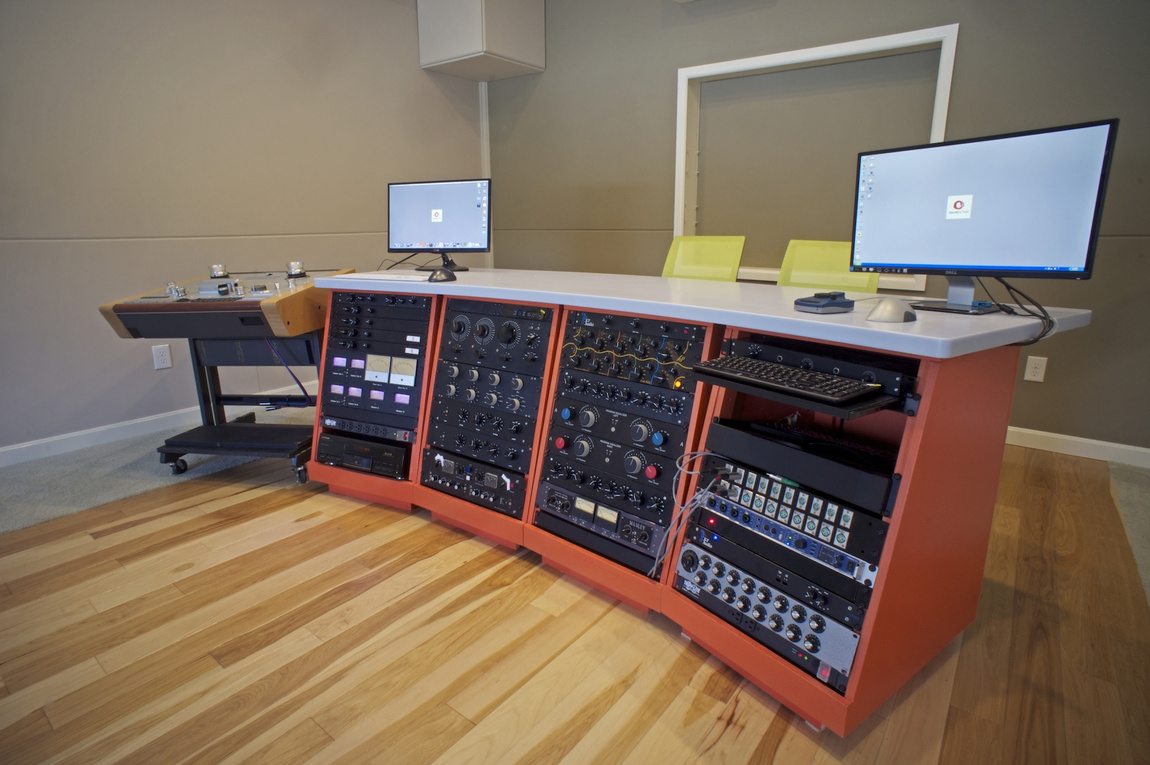
\includegraphics[width=1\textwidth]{sunnystudio}
	\end{figure}
	
Most of this equipment is designed, assembled and tested in collaboration with JCF audio's founder and owner, Joshua Florian \cite{florian2015}. After Nam and Florian worked together at LA's Mastering Lab, Nam came to value Florian's understanding of what they describe as ``yester-tech'' \cite{florian2015b}: older audio hardware circuit designs, usually discrete semiconductor or tube, that were used in high end recording and mastering studios along with the rise and heyday of major labels. A number of parts in Nam's current setup come from A\&R mastering studio, which he purchased when they closed down. 



This section does not contain a particular product description. However, the concept of ``yester-tech'' is, perhaps understatedly, at the bottom of the discussion on open-source hardware. Open-source is mostly defined in opposition to closed-source or proprietary information, the privacy of which is legally defended by its inventors and implementors. However, mu

For hardware, this information details the designs of devices, and in most technological economies, this intellectual property is legally protected by copyright, patents. Legally, these expire or have limitations allowing people today to rightfully build and sell their own version of, for example, the API 2520 that Nam mentions in his interview. 

The goals of including comments stemming from my discussion with Nam were simple: prove that secretive designers are still able to succesfully build businesses out of their expertise, expose their use of open-source designs, if any, and that simply taking from publicly available designs was itself a way to perpetuate its importance. In other words, open-source hardware design is a robust practice. 

\section{Design comments}

All these projects constitute a limited sample of the ideas driving innovation in the field of electronic music hardware. Through them, we've explored a significant amount of the space of possibilities defined in the first chapter by the components available. They  Primary sources range from highly formatted peer review journals to unstable forum posts, mired with dead links and noise.  

%Rather than trying 

% ---------------
% To incorporate in this chapter

\begin{unsortedStuff}	
\section*{(TO INCORPORATE)}
	\begin{itemize}
		\item 
	\end{itemize}
\end{unsortedStuff}
		
%Blank page to add written thoughts
\begin{optBlankSpace}
	\newpage
	\mbox{}
\end{optBlankSpace}

